\section{Hot tap water profile}

% The D.H.W does not match between profile and year annual consumption.
	
Since september 26, 2015, the Ecodesign \cite{Ecodesign} and energy labeling guidelines,also apply to appliances for the production of domestic hot water. 
Devices that do not comply with these guidelines may no longer be sold. In figure \ref{fig:energylabel} the tap water profile label has been highlighted with red square.\\
	
	
\begin{figure}[H]
	\centering
	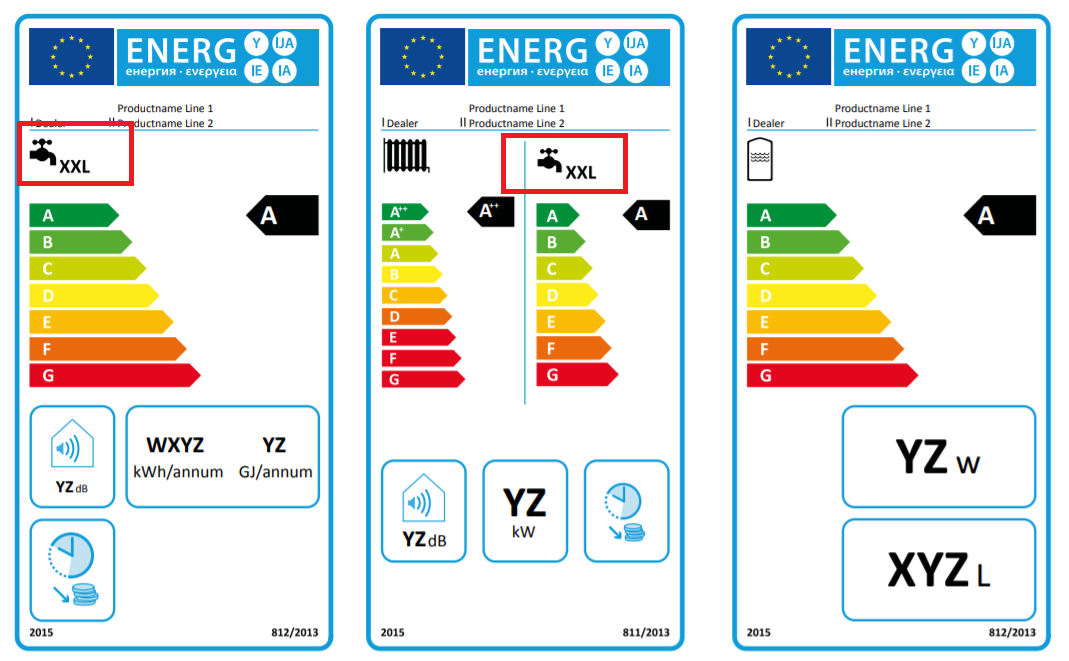
\includegraphics[width=1\columnwidth]{pictures/energy label.png}
	\caption[Short title]{Energy label[ \cite{Ecodesign}}
	\label{fig:energylabel}
\end{figure}

The hot water classes are defined in the EU regulation with different category label. For example hot water class with label "XL" must be able to supply 18 kWh of hot water per day (1 kWh corresponds to 64.8 MJ heat). This EU regulation also stipulates what conditions hot tap water class must be met.
Figure 8 show that tap water profile for showering can only be selected from label S to XXL.
	
\begin{figure}[ht]
	\centering
	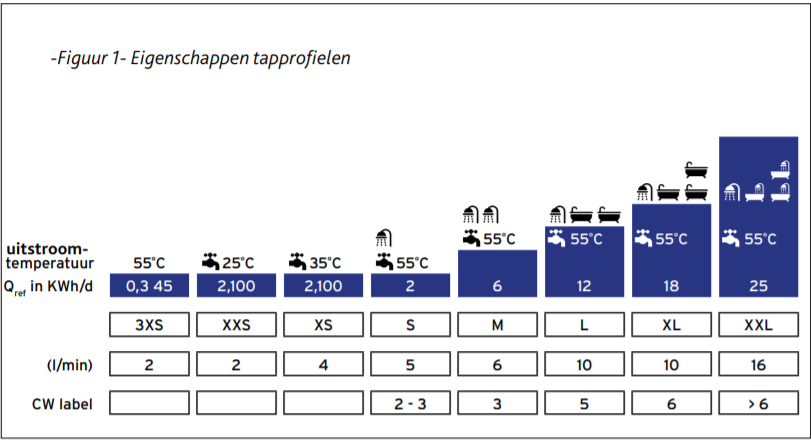
\includegraphics[width=1\columnwidth]{pictures/tap profile.png}
	\caption[Short title]{hot water profile labels \cite{Ecodesign}.}
	\label{fig:profilelabels}
\end{figure}
	
	
\begin{figure}[H]
	\centering
	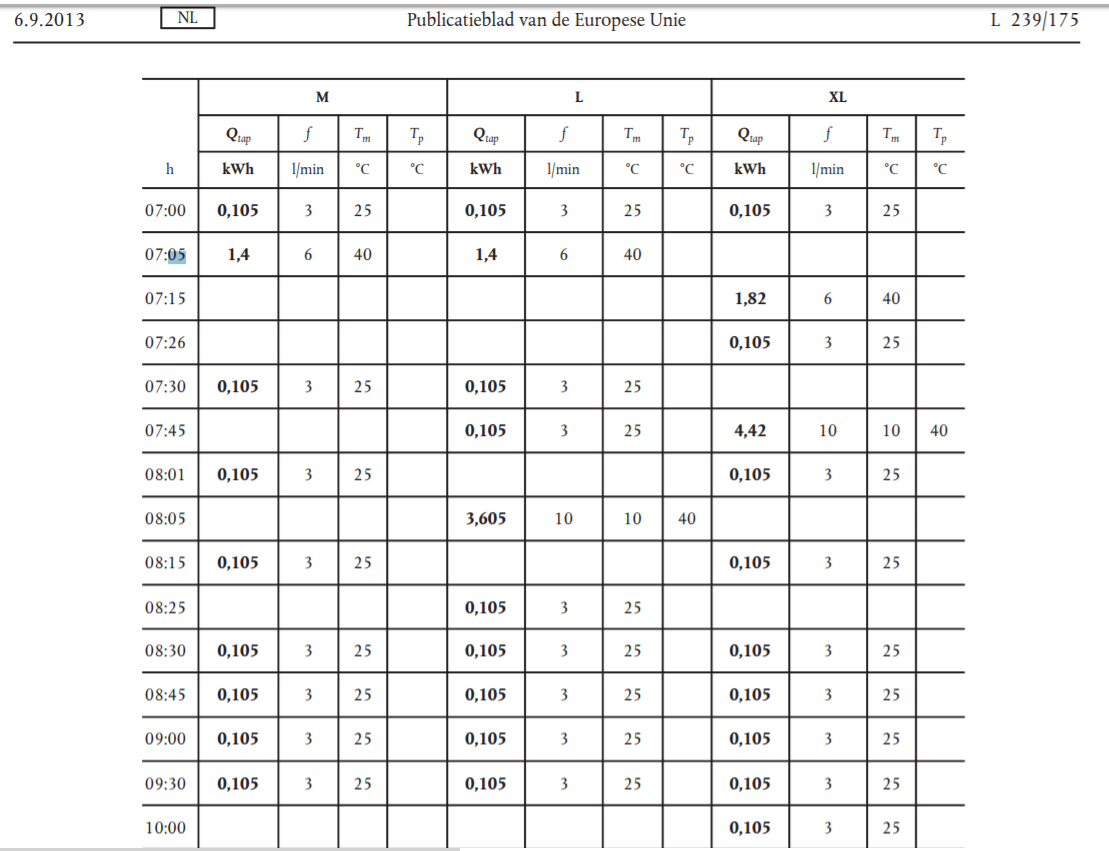
\includegraphics[width=1\columnwidth]{pictures/Profile_M1.png}
	\caption[Short title]{Capaciteitsprofielen van waterverwarmingstoestellen.}
	\label{fig:capaciteitM1}
\end{figure}
	
\begin{figure}[H]
	\centering
	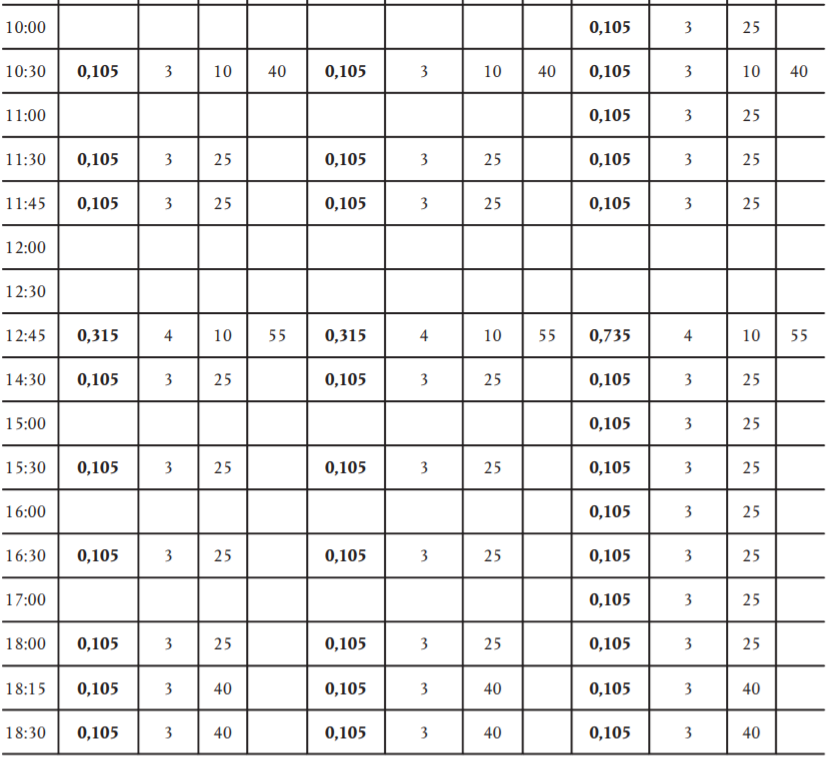
\includegraphics[width=1\columnwidth]{pictures/Profile_M2.png}
	\caption[Short title]{Capaciteitsprofielen van waterverwarmingstoestellen.}
	\label{fig:capaciteitM2}
\end{figure}
	
\begin{figure}[H]
	\centering
	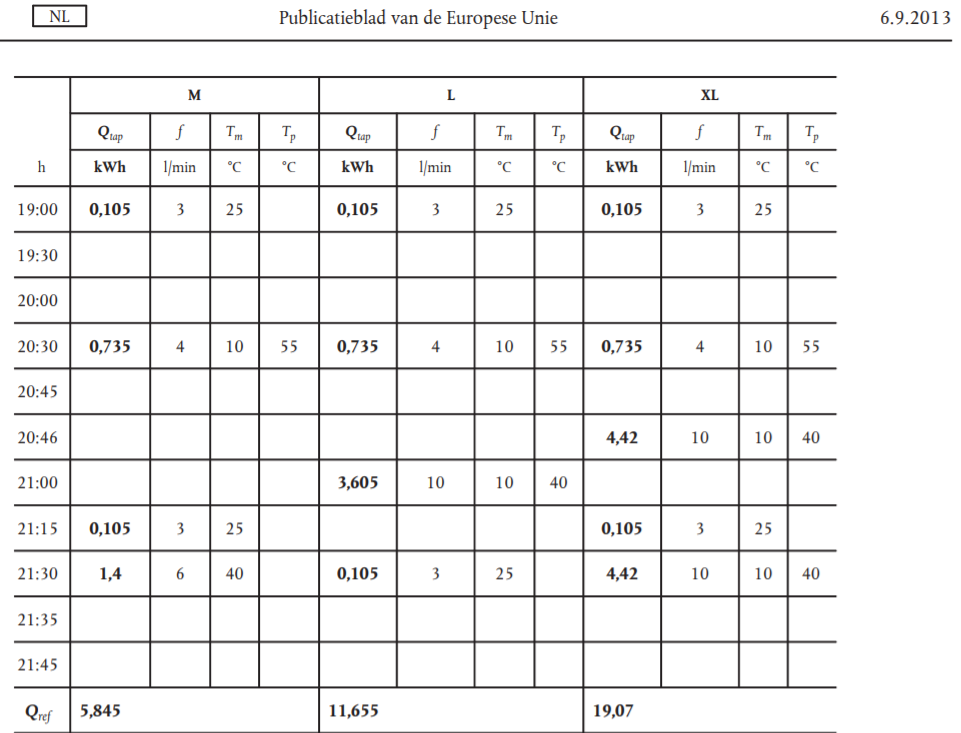
\includegraphics[width=1\columnwidth]{pictures/Profile_M3.png}
	\caption[Short title]{Capaciteitsprofielen van waterverwarmingstoestellen.}
	\label{fig:capaciteitM3}
\end{figure}
	